\documentclass[dvipdfmx]{beamer}
\usepackage{tutorial}

\title{計算機実験(付録)}
\date{2016}

\begin{document}

\begin{frame}
  \titlepage
  \tableofcontents
\end{frame}

\section{代数方程式の解法}

\begin{frame}[t,fragile]{代数方程式}
  \begin{itemize}
    \setlength{\itemsep}{1em}
  \item 実係数の$n$次方程式
    \[
    P(z) = z^n + a_1 z^{n-1} + \cdots + a_n = 0
    \]
  \item ニュートン法 + 減次 (次数低下法)
    \begin{itemize}
    \item ニュートン法により一つの解($\alpha$)を求める
    \item $g(x) = f(x) / (x-\alpha)$の解として、他の解を逐次求めていく
    \item 毎回誤差がたまっていくため、解はくずれていく
    \end{itemize}
  \end{itemize}
\end{frame}


\begin{frame}[t,fragile]{Durand-Kerner-Aberth法 (Wierstrass法)}
  \begin{itemize}
    \setlength{\itemsep}{1em}
  \item 真の解を$\alpha_1,\alpha_2,\cdots,\alpha_n$とすると
    \[
    P(z) = (z-\alpha_1) (z-\alpha_2) \cdots (z-\alpha_n)
    \]
  \item $\alpha_1,\alpha_2,\cdots,\alpha_n$に現在の近似解$z^{(\nu)}_1,z^{(\nu)}_2,\cdots,z^{(\nu)}_n$を代入し、$z=z^{(\nu)}_k$における微分の値を評価
    \[
    P'(z^{(\nu)}_k) \approx \prod_{j \ne k} (z^{(\nu)}_k - z^{(\nu)}_j)
    \]
  \item ニュートン法による反復
    \[
    z^{(\nu+1)}_k = z^{(\nu)}_k - \frac{P(z^{(\nu)}_k)}{\prod_{j \ne k} (z^{(\nu)}_k - z^{(\nu)}_j)}
    \]
  \end{itemize}
\end{frame}

\begin{frame}[t,fragile]{初期値の選び方}
  \begin{itemize}
    \setlength{\itemsep}{1em}
  \item ある十分に大きな実数$r_0$を用いて
    \[
    z^{(0)}_k = - \frac{a_1}{n} + r_0 \exp \Big[ i \Big( \frac{2(k-1)\pi}{n} + \frac{\pi}{2n} \Big) \Big]
    \]
    複素平面上の中心$-a_1/n$、半径$r_0$の円周上の等間隔の点
  \item DKA法の収束
    \begin{itemize}
    \item $r_0$が十分大きい時
      \[\hspace*{-4cm} z^{(1)}_k + \frac{a_1}{n} \approx (1-\frac{1}{n}) (z^{(0)}_k + \frac{a_1}{n})
      \]
    \item 解の近傍では二次収束
    \item 解は互いに反発
    \item 例: $z^5-10z^4+43z^3-104z^2+150z-100=0$ (山本2003)
    \end{itemize}
  \end{itemize}
  \vspace*{-3.7cm}\hspace*{7.5cm}
  \resizebox{.3\textwidth}{!}{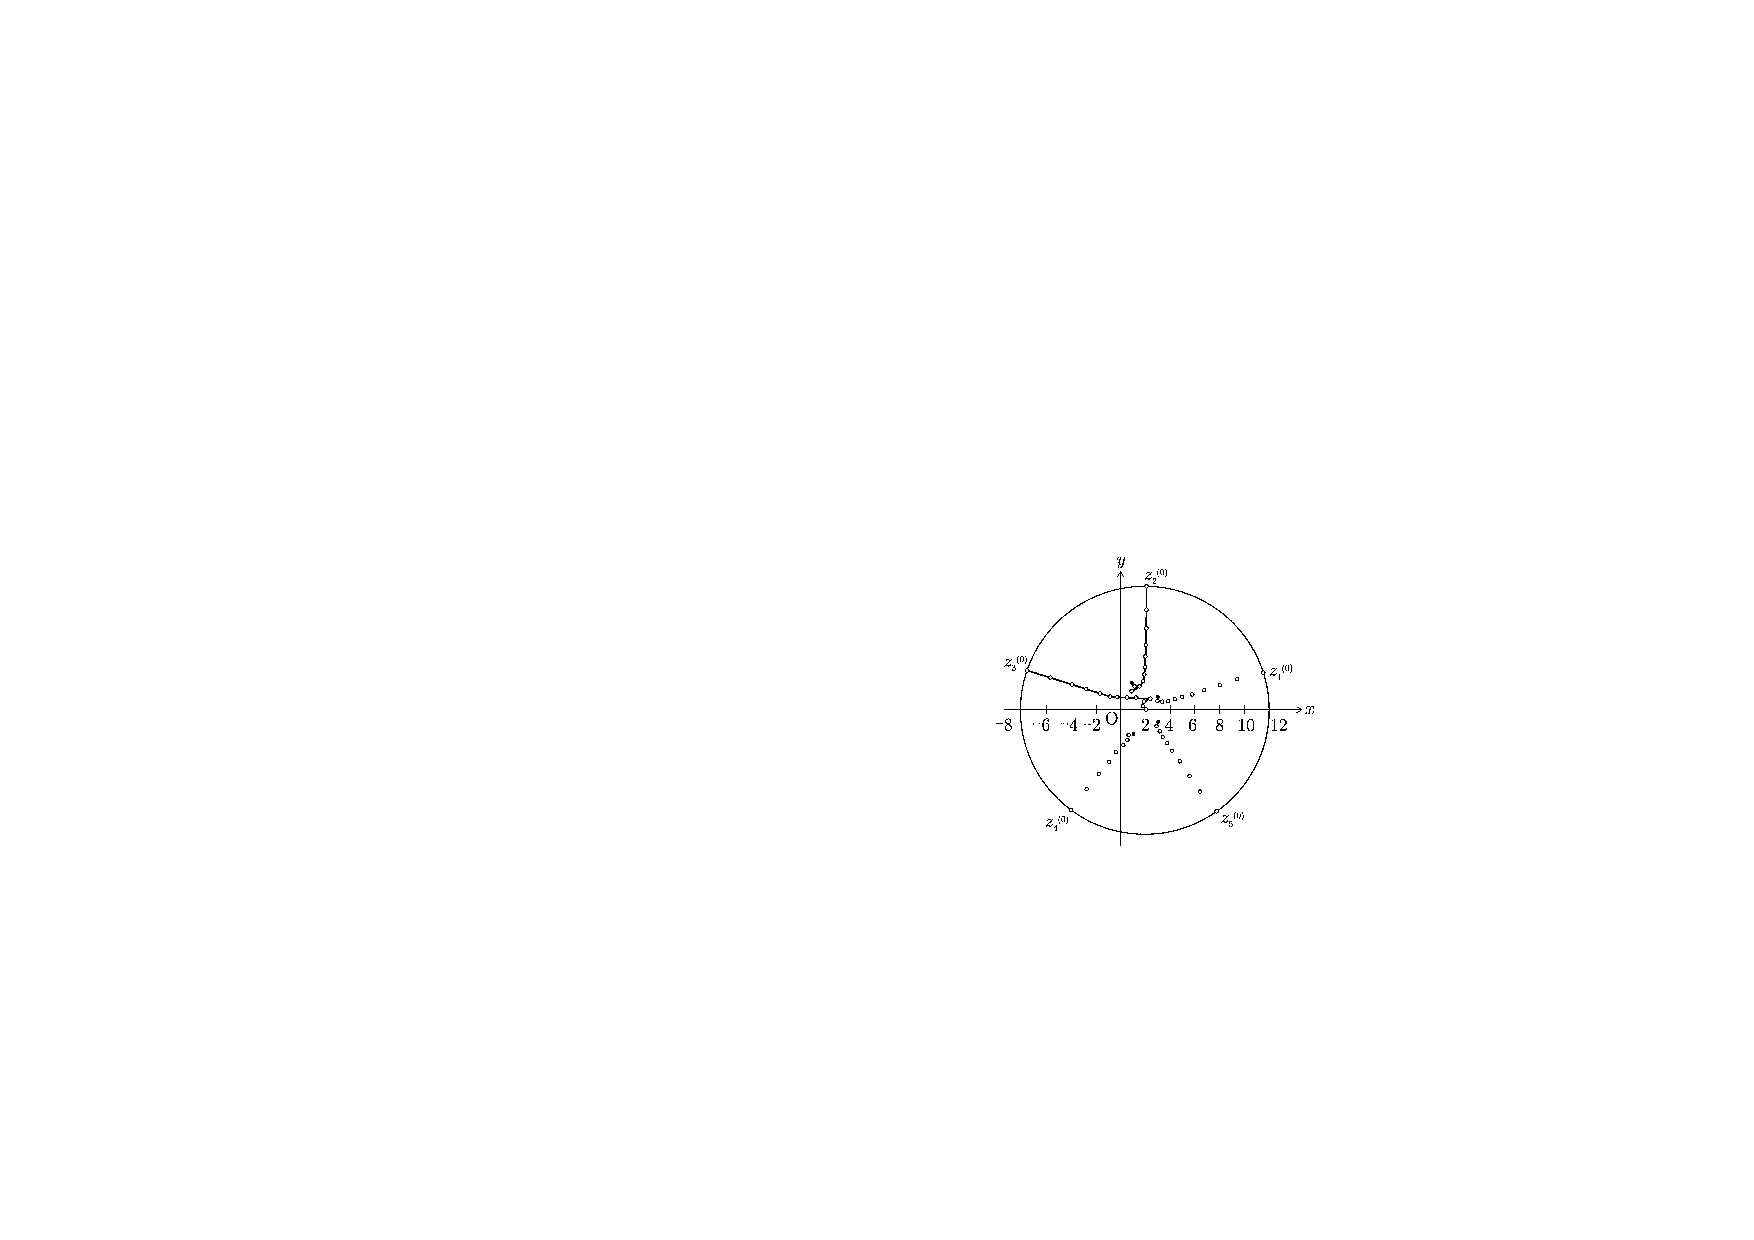
\includegraphics{image/DKA.pdf}}
\end{frame}

\section{Numerov法}

\begin{frame}[t,fragile]{時間依存しないシュレディンガー方程式}
  \begin{itemize}
    \setlength{\itemsep}{1em}
  \item 井戸型ポテンシャル中の一粒子問題
    \begin{align*}
      \big[ -\frac{\hbar^2}{2m}\frac{d^2}{dx^2} + V(x) \big] \psi(x) = E \psi(x) \\
      V(x) = \begin{cases}
        0 & \text{$a \le x \le b$} \\ \infty & \text{otherwise}
      \end{cases}
    \end{align*}
  \item $\hbar^2/2m = 1$、$a=0$、$b=1$となるように変数変換して
    \begin{align*}
      \big( \frac{d^2}{dx^2} + E \big) \psi(x) = 0 \qquad 0 \le x \le 1
    \end{align*}
    を境界条件$\psi(0) = \psi(1) = 0$のもとで解けば良い
  \end{itemize}
\end{frame}

\begin{frame}[t,fragile]{微分方程式の積分による解法}
  \begin{itemize}
    \setlength{\itemsep}{1em}
  \item Numerov法
    \begin{itemize}
    \item 二階の常微分方程式で一階の項がない場合に使える
    \item 4次の陰解法
    \item 方程式が線形の場合は陽解法に書き直せる
    \end{itemize}
  \item 微分方程式
    \[
    \frac{d^2y}{dx^2} = f(x,y)
    \]
  $y=y(x)$を$x=x_i$のまわりでテイラー展開する。$x_{i \pm 1} = x_i \pm h$での表式は
      \[
      y(x_{i+1}) = y(x_i) \pm h y'(x_i) + \frac{h^2}{2} y''(x_i) \pm \frac{h^3}{6} y'''(x_i) + \frac{h^4}{24} y''''(x_i)  + O(h^5)
      \]
  \end{itemize}
\end{frame}

\begin{frame}[t,fragile]{Numerov法}
  \begin{itemize}
    \setlength{\itemsep}{1em}
  \item 二階微分の差分近似 ($y_i \equiv y(x_i)$等と書く)
    \[
    \frac{y_{i+1} - 2 y_i + y_{i-1}}{h^2} = y''_{i} + \frac{h^2}{12} y''''_{i} + O(h^4)
    \]
  一方で、微分方程式より
    \[
    y''''_i = \frac{d^2f}{dx^2}\Big|_{x=x_i} = \frac{f_{i+1}-2f_i+f_{i-1}}{h^2} + O(h^2)
    \]
    組み合わせると
    \[
    y_{i+1} = 2y_i - y_{i-1} + \frac{h^2}{12} (f_{i+1} + 10f_{i} + f_{i-1}) + O(h^6)
    \]
  \end{itemize}
\end{frame}

\begin{frame}[t,fragile]{Numerov法}
  \begin{itemize}
    \setlength{\itemsep}{1em}
  \item 方程式が線形の場合、$f(x,y) = -a(x) y(x)$を代入すると
    \[
    y_{i+1} = 2y_i - y_{i-1} - \frac{h^2}{12} (a_{i+1}y_{i+1} + 10a_{i}y_{i} + a_{i-1}y_{i-1}) + O(h^6)
    \]
  $y_{i+1}$を左辺に集めると、陽解法となる
    \[
    y_{i+1} = \frac{2 (1-\frac{5h^2}{12} a_i)y_i - (1 + \frac{h^2}{12} a_{i-1}) y_{i-1}}{1 + \frac{h^2}{12} a_{i+1}} + O(h^6)
    \]
  \end{itemize}
\end{frame}

\begin{frame}[t,fragile]{Numerov法による固有値問題の解法}
  \begin{itemize}
    \setlength{\itemsep}{1em}
  \item $x_i=h \times i$ ($h=1/n$)、$x_0=0$、$x_n=1$とする
  \item $\psi(x_0)=0$、$\psi(x_1) = 1$を仮定 ($\psi'(x_0)=1/h$と与えたことに相当)
  \item $E = 0$とおく
  \item Numerov法を用いて、$x=x_n$まで積分
  \item $\psi(x_n)$の符号がかわるまで、$E$を少しずつ増やす
  \item 符号が変わったら、$E$の区間を半分ずつに狭めていき、$\psi(x_n)=0$となる$E$ (固有エネルギー)と$\psi(x)$ (波動関数)を得る
  \end{itemize}
\end{frame}

\section{実習0}

\begin{frame}[t,fragile]{EX0-1: 実習環境の準備}
  \begin{itemize}
    \setlength{\itemsep}{1em}
  \item[0-1-1] ECCS端末(iMac)を利用する場合
    \begin{itemize}
    \item ログイン
    \item 「ターミナル」を開く
    \end{itemize}
  \item[0-1-2] MateriApps LIVE!を利用する場合
    \begin{itemize}
    \item MateriApps LIVE! のインストール・設定(\href{https://github.com/cmsi/MateriAppsLive/wiki/MateriAppsLive-ltx}{README.html}、\href{http://www.slideshare.net/cms_initiative/materiapps-live-52477264}{malive.pdf})
    \item スタートメニュー⇒「Accessories」⇒「LXTerminal」
    \end{itemize}
  \item[0-1-3] ハンドブック 2章 UNIX入門
    \begin{itemize}
    \item 2.1 UNIXのコマンド (2.1.1)
    \item 2.2 リモートログインとファイル転送
    \item 2.3 Emacsを使う (2.3.2) (viを使ってもよい)
    \item 2.4 Gnuplotを使う
    \end{itemize}
  \end{itemize}
\end{frame}

\begin{frame}[t,fragile]{EX0-2: C言語と\LaTeX の練習}
  \begin{itemize}
    %\setlength{\itemsep}{1em}
  \item[0-2-1] \href{https://github.com/todo-group/computer-experiments/blob/master/exercise/basics/hello.c}{exercise/basics/hello.c}をCコンパイラでコンパイルし、実行
  \item[0-2-2] ハンドブック 3章 C言語入門
    \begin{itemize}
    \item 3.1 C言語の基礎知識 (3.1.1, 3.1.2, 3.1.3)
    \item 3.2 制御文 (3.2.1, 3.2.2)
    \item 3.6 関数 (3.6.2)
    \end{itemize}
  \item[0-2-3] \href{https://github.com/todo-group/computer-experiments/blob/master/exercise/basics/hello.tex}{exercise/basics/hello.tex}を{\tt platex}コマンドと{\tt dvipdfmx}コマンドを使ってPDFファイルに変換
  \item[0-2-4] ハンドブック 4章 \LaTeX 入門
    \begin{itemize}
    \item 4.1 \LaTeX の実行
    \end{itemize}
  \item[0-2-5] Gnuplotを使い、$\sin$関数をプロットし、PostScript形式でファイル(*.eps)に出力(ハンドブック2.4節)。作成した図のファイルを \LaTeX に張り込み、PDFファイルを作成(ハンドブック4.8節)
  \end{itemize}
\end{frame}

\section{実習1}

\begin{frame}[t,fragile]{EX1-1: フィボナッチ数列、数値微分、ニュートン法}
  \begin{itemize}
    \setlength{\itemsep}{1em}
  \item[1-1-1] フィボナッチ数列($a_{n+2}=a_{n+1}+a_n$ ($n \ge 0$), $a_0=0$, $a_1=1$)を計算するプログラムを作成し、$a_{20}$, $a_{30}$, $a_{40}$, $a_{50}$, $a_{60}$を求めよ。桁あふれに注意すること。結果は、\LaTeX の{\tt tabular}環境を使って表にまとめよ
  \item[1-1-2] $f(x)=\sin x$について、$x=0.3\pi$における$f'(x)$の値を数値微分により計算するプログラムを作成せよ。数値微分の刻みを$h=1,1/2,1/4,1/8,\cdots$と減少させていった時、誤差がどのように振る舞うか図示せよ
  \item[1-1-3] $\sqrt[3]{x}$を求めるNewtonの反復式を書け。これを用いて、$\sqrt[3]{10}$を求めるプログラムを作成せよ。反復にしたがって、値がどのように真値に近づいていくか図示せよ
  \end{itemize}    
\end{frame}

\begin{frame}[t,fragile]{EX1-2: 代数方程式の解}
  \begin{itemize}
    \setlength{\itemsep}{1em}
  \item[1-2-1] 次数低下法を用いて、代数方程式の全ての解を求めるプログラムを作成せよ
  \item[1-2-2] Durand-Kerner-Aberth法を用いて、代数方程式の全ての解を求めるプログラムを作成せよ。方程式の次数を増やすにつれ、収束までにかかる時間がどのように増えるか調べよ
  \end{itemize}    
\end{frame}

\begin{frame}[t,fragile]{EX1-3: C言語におけるポインタと配列}
  \begin{itemize}
    \setlength{\itemsep}{1em}
  \item[1-3-1] \verb+double m[10][10];+ で宣言されたCの二次元配列について、\verb^*(m+2)[3]^ と \verb^(*(m+2))[3]^ はそれぞれどの要素の値を返すか? なぜこの2つは異なる要素の値を返すのか?
  \item[1-3-2] C言語におけるポインタの振る舞いをテストするプログラム(\href{https://github.com/todo-group/computer-experiments/blob/master/exercise/linear_system/pointer.c}{exercise/linear\_system/pointer.c})のソースコードを見て、どのような出力が生成されるか予想せよ。実際にコンパイル・実行して予想を確かめてみよ
  \end{itemize}
\end{frame}

\section{実習2}

\begin{frame}[t,fragile]{EX2-1: 常微分方程式の初期値問題}
  \begin{itemize}
    \setlength{\itemsep}{1em}
  \item[2-1-1] 空気による摩擦のあるバネの問題を考える。壁にバネが繋が
    れ、バネの先には質量$m$の物体が繋がっている。床との摩擦は考えない
    ものとする。バネの伸びる方向に$x$座標を取り、自然長の位置を原点と
    すると、物体の運動方程式は以下のように与えられる。
    \[
    m\frac{\mathrm{d} ^2x}{\mathrm{d} t^2} = -kx - \kappa \frac{\mathrm{d} x}{\mathrm{d} t} 
    \]
    ここで、$k$はバネ定数、$\kappa$は摩擦の比例定数とする。Euler法を使い$x(t)$を30 [sec]まで計算せよ。その際、刻み幅$h$の大きさを変化させ、解の変わる様子を確認せよ。ただし、$k$ = 2 [N/m], $\kappa$ = 0.2 [kg/sec]、$m$ = 1 [kg]、初期条件は$x(0)$ = 10 [m]、$x'(0)$ = 0 [m/sec] とする
  \end{itemize}
\end{frame}

\begin{frame}[t,fragile]{EX2-2: 高次の解法}
  \begin{itemize}
    \setlength{\itemsep}{1em}
  \item[2-2-1] 中点法、3次のRunge-Kutta法、4次のRunge-Kutta法を用いて同様の計算を行い、精度の向上の様子を調べよ
  \item[2-2-2] 空気抵抗も床との摩擦も無い場合についてシミュレーションを行い、全エネルギー(運動エネルギーとポテンシャルエネルギーの和)の時間変化の様子を観察せよ。なぜ、全エネルギーが保存しないのか? 一方で、ある一定の誤差の範囲内で全エネルギーを保存する手法として、Symplectic法が知られている。この方法について調べ、実際にプログラムを作成し、シミュレーション結果について考察せよ
  \end{itemize}
\end{frame}

\section{実習その3}

\begin{frame}[t,fragile]{EX3-1: サンプルプログラムの実行}
  \begin{itemize}
    %\setlength{\itemsep}{1em}
  \item[3-1-1] ガウスの消去法のサンプルプログラム(\href{https://github.com/todo-group/computer-experiments/blob/master/exercise/linear_system/gauss.c}{exercise/linear\_system/gauss.c})をコンパイル・実行せよ。実行時にコマンドライン引数に行列の内容が書かれたファイル名({\tt input1.dat})を指定する必要があることに注意
\begin{lstlisting}
$ cc gauss.c -o gauss
$ ./gauss input1.dat
\end{lstlisting}
  \item[3-1-2] LU分解のサンプルプログラム(\href{https://github.com/todo-group/computer-experiments/blob/master/exercise/linear_system/lu_decomp.c}{exercise/linear\_system/lu\_decomp.c})をコンパイル・実行せよ。コンパイル時にLAPACKをリンク({\tt -llapack})する必要があることに注意(ハンドブック3.1.6節)
\begin{lstlisting}
$ cc lu_decomp.c -o lu_decomp -llapack
$ ./lu_decomp input1.dat
\end{lstlisting}
  \end{itemize}
\end{frame}

\begin{frame}[t,fragile]{EX3-2: ピボット選択、境界条件}
  \begin{itemize}
    %\setlength{\itemsep}{1em}
  \item[3-2-1] {\tt gauss.c}では、ピボット選択を行っていないため、入力が{\tt input2.dat}の場合には正しい解が得られない。ピボット選択を行うよう{\tt gauss.c}を修正せよ
  \item[3-2-2] \href{https://github.com/todo-group/computer-experiments/blob/master/exercise/linear_system/laplace_lu.c}{exercise/linear\_system/laplace\_lu.c}では、ディリクレ型の境界条件[$u(0,y) = \sin(\pi y)$, $u(x,0)=u(x,1)=u(1,y)=0$]のもとでのラプラス方程式の解をLU分解により求めている。境界条件を変えてみて解がどのように変化するか、Gnuplotを用いてプロットして確認せよ(Gnuplotの{\tt splot}コマンドを使う)
  \end{itemize}
\end{frame}

\begin{frame}[t,fragile]{EX3-3: ヤコビ法、ガウス・ザイデル法、SOR法}
  \begin{itemize}
    %\setlength{\itemsep}{1em}
  \item[3-3-1] \href{https://github.com/todo-group/computer-experiments/exercise/blob/master/linear_system/laplace_jacobi.c}{exercise/linear\_system/laplace\_jacobi.c}は、作りかけのヤコビ法のプログラムである。収束判定のコードを追加し、プログラムを完成せよ。計算結果や計算速度を{\tt laplace\_lu.c}と比較せよ
  \item[3-3-2] ヤコビ法のプログラム({\tt lapalace\_jacobi.c})を元に、ガウス・ザイデル法、SOR法のプログラムを作成せよ。収束までの回数を比較せよ。
特にSOR法の場合、パラメータ$\omega$の選び方により、どのように収束回数が変化するか観察し、最適な$\omega$の値について考察せよ
  \end{itemize}
\end{frame}

\section{実習その4}

\begin{frame}[t,fragile]{EX4-1: ハウスホルダー法とべき乗法}
  \begin{itemize}
    %\setlength{\itemsep}{1em}
  \item[4-1-1] ハウスホルダー法による対角化のサンプルプログラム(\href{https://github.com/todo-group/computer-experiments/blob/master/exercise/eigenvalue_problem/diag.c}{exercise/eigenvalue\_problem/diag.c})をコンパイル・実行せよ
\begin{lstlisting}
$ cc diag.c -o diag
$ ./diag input1.dat
\end{lstlisting}
\item[4-1-2] {\tt diag.c}により得られた固有ベクトルが互いに正規直交していることを確認するコードを作成し実行せよ(それぞれの固有ベクトルを行とする行列とその転置行列をかけて、単位行列になることを確認すればよい)
  \item[4-1-3] \href{https://github.com/todo-group/computer-experiments/blob/master/exercise/eigenvalue_problem/power.c}{exercise/eigenvalue\_problem/power.c}は、べき乗法により最大固有ベクトルを計算するプログラムである(ただし、プログラムは未完成)。62行目に固有値を計算するコードを追加せよ。結果がEX4-1-1の最大固有値と一致するかどうか確認せよ
  \end{itemize}
\end{frame}

\begin{frame}[t,fragile]{EX4-2: 特異値分解}
  \begin{itemize}
    %\setlength{\itemsep}{1em}
  \item[4-2-1] 特異値分解のサンプルプログラム(\href{https://github.com/todo-group/computer-experiments/blob/master/exercise/eivenvalue_problem/svd.c}{exercise/eigenvalue\_problem/svd.c})をコンパイル・実行せよ。入力{\tt matrix1.dat}を用いて、結果を確認せよ
\begin{lstlisting}
$ cc svd.c -o svd -llapack -lm
$ ./svd matrix1.dat
\end{lstlisting}
  \item[4-2-2] 完全特異値分解を行うサンプルプログラム(\href{https://github.com/todo-group/computer-experiments/blob/master/exercise/eivenvalue_problem/full_svd.c}{exercise/eivenvalue\_problem/full\_svd.c})をコンパイル・実行せよ。{\tt svd.c}との違いを{\tt diff}コマンドを使って調べよ。
  \end{itemize}
\end{frame}

\begin{frame}[t,fragile]{EX4-3: 二重井戸ポテンシャル中の粒子}
  \begin{itemize}
    %\setlength{\itemsep}{1em}
  \item[4-3-1] \href{https://github.com/todo-group/computer-experiments/blob/master/exercise/eigenvalue_problem/double_well.c}{exercise/eigenvalue\_problem/double\_well.c}は、対角化により、有限の障壁で隔てられた二重井戸ポテンシャル中の粒子
    \begin{equation*}
      V(x) = \begin{cases}
        \infty & x < 0, \ x > 1 \\
        0 & 0 < x < \frac{1}{2} - w, \ \frac{1}{2}+w < x < 1 \\
        v & \frac{1}{2} - w < x < \frac{1}{2}+w
      \end{cases}
    \end{equation*}
    の固有値と固有ベクトルを計算するプログラムである。コマンドライン引数として、刻み数{\tt n}、障壁の高さ{\tt v}、障壁の幅{\tt width}を指定する。障壁の幅や高さを変えた時に固有値や固有ベクトルがどのように変化するか調べ、図示せよ。また、その物理的意味を考察せよ。(ヒント: 障壁が無限に高い極限からの摂動を考えてみよ)
  \end{itemize}
\end{frame}

\begin{frame}[t,fragile]{EX4-4: Lanczos法}
  \begin{itemize}
    %\setlength{\itemsep}{1em}
  \item[4-4-1] Lanczos法により固有値を計算するプログラムを作成せよ。Ritz値が、繰り返しに従ってどのように振る舞うか図示してみよ
  \item[4-4-2] EX4-2-1の行列は疎行列(三重対角行列)である。その性質を利用して、行列ベクトル積を効率的に計算するコードを作成し、べき乗法あるいはLanczos法に組み込み、その速度を計測せよ
  \end{itemize}
\end{frame}

\begin{frame}[t,fragile]{EX4-5: 行列の低ランク近似}
  \begin{itemize}
    %\setlength{\itemsep}{1em}
  \item[4-5-1] {\tt svd.c}の最後では行列のランク$[{\rm min}(m,n)-1]$近似を計算している。コマンドライン引数で近似のランク数を指定できるように、また近似の誤差(フロベニウスノルム)を計算・出力するようプログラムを修正せよ。{\tt matrix2.dat}、{\tt matrix3.dat}について、近似度合いを変えながら、その出力を観察せよ
  \item[4-5-2] {\tt svd.c}中のLAPACKの特異値分解{\tt dgesvd}の呼び出し(54行目)では、行列の次元({\tt m}と{\tt n})、左特異ベクトル({\tt u})と右特異ベクトル({\tt vt})の順番が、もともとの{\tt dgesvd}の\href{http://www.netlib.org/lapack/explore-html/d8/d2d/dgesvd_8f.html}{ドキュメント}とは逆になっている。このプログラムが正しく動作するのはなぜか?
  \end{itemize}
\end{frame}

\begin{frame}[t,fragile]{EX4-6: 応用課題}
  \begin{itemize}
    %\setlength{\itemsep}{1em}
  \item[4-6-1] {\tt double\_well.c}では全ての変数が無次元化されている。粒子の質量、井戸の幅、障壁の幅、高さとして、(次元をもつ)物理的に妥当な値を仮定せよ。それらを無次元化すると、{\tt v}、{\tt width}の値はいくらになるか? また、それらの値から{\tt double\_well.c}により計算された固有値を、次元をもつ実際の値に換算してみよ
  \item[4-6-2] 入力{\tt input1.txt}はFrank行列と呼ばれる行列で、全ての固有値を解析的に求めることができる。一般の次元のFrank行列の固有値がどのように求められるか調べよ。Frank行列のように固有値が解析的に計算できる密行列には他にどのようなものがあるか?
  \item[4-6-3] 画像ファイルを行列形式に変換し、SVDで圧縮してみよ。どの程度まで圧縮可能か?
  \end{itemize}
\end{frame}

\section{カーネル法}

\begin{frame}[t,fragile]{カーネルトリック}
  \begin{itemize}
    %\setlength{\itemsep}{1em}
  \item 方程式を変形 ${\bf w} = \frac{1}{\lambda} \Phi^{\rm t} ({\bf y} -\Phi {\bf w})$
  \item $\alpha = \frac{1}{\lambda}({\bf y} -\Phi {\bf w})$と定義すると${\bf w} =\Phi^{\rm t} \alpha$
    \item $w$は$\begin{pmatrix} \phi_1(x_1) \\ \vdots \\ \phi_M(x_1) \end{pmatrix} \cdots 
      \begin{pmatrix} \phi_1(x_N) \\ \vdots \\ \phi_M(x_N) \end{pmatrix}$の線形結合
    \item $M$次元中の$N$次元部分空間にある ($M$: 基底関数の数、$N$: サンプル数)
    \item 基底関数を増やしても自由度は増えない
    \item $w$を求める代わりに、直接$\alpha$を求めても良い (リプリゼンター定理)
  \end{itemize}
\end{frame}

\begin{frame}[t,fragile]{カーネルによる線形回帰}
  \begin{itemize}
    %\setlength{\itemsep}{1em}
  \item 残差$R$を$\alpha$をつかって表現
    \[
    R(\alpha) = | y - \Phi \Phi^{\rm t} \alpha |^2 + \lambda \alpha^{\rm t} \Phi \Phi^{\rm t} \alpha
    \]
  \item グラム行列(Gram matrix) $K \equiv \Phi \Phi^{\rm t}$を導入すると
    \[
    R(\alpha) = | y - K \alpha |^2 + \lambda \alpha^{\rm t} K \alpha
    \]
  \item グラム行列($N \times N$対称行列)の成分
    \[
    K_{ik} = \sum_j \Phi_{ij} \Phi_{kj} = \sum_j \phi_j(x_i) \phi_j(x_k) \equiv {\color{red} k(x_i,x_k)}
    \]
  \item $M$個の基底関数の組を考えるかわりに1つのカーネル関数$k(x,x')$を導入すればよい(カーネル法)
  \end{itemize}
\end{frame}

\begin{frame}[t,fragile]{カーネルによる線形回帰}
  \begin{itemize}
    %\setlength{\itemsep}{1em}
  \item 残差$R$の最小化
    \[
    \alpha = (K + \lambda \, {\rm I})^{-1} {\bf y}
    \]
  \item 点$x$における$y$の推定値
    \begin{align*}
    y &= \sum_j \phi_j(x) w_j = \sum_{i,j} \phi_j(x) \phi_j(x_i) \alpha_i = \sum_i k(x_i,x) \alpha_i \\ &= k^{\rm t}(x) \alpha = k^{\rm t}(x) (K + \lambda \, {\rm I})^{-1} {\bf y}
k(x) = \begin{pmatrix} k(x_1,x) \\ k(x_2,x) \\ \vdots \\ k(x_N,x) \end{pmatrix}
    \end{align*}
  \item 例: ガウシアンカーネル $k(x,x') = \exp(-\beta|x-x'|^2)$
  \end{itemize}
\end{frame}

\section{実習その5}

\begin{frame}[t,fragile]{EX5-1: 最小二乗フィッティング}
  \begin{itemize}
    %\setlength{\itemsep}{1em}
  \item[5-1-1] \href{https://github.com/todo-group/computer-experiments/blob/master/exercise/linear_regression/regression.c}{exercise/linear\_regression/regression.c}は数値データを読み込み、一次式で最小二乗フィッテイングを行うプログラムである。実行すると最終行に一次式の係数が出力される。
\begin{lstlisting}
$ ./regression measurement1.dat
\end{lstlisting}
    ファイル{\tt measurement1.dat}の1カラム目は$x$、2カラム目は$y$、3カラム目は$y$の誤差の値(計算の中では使っていない)である。元データとフィッティング結果をグラフにせよ
  \end{itemize}
\end{frame}

\begin{frame}[t,fragile]{EX5-2: 高次関数でのフィッティング}
  \begin{itemize}
    %\setlength{\itemsep}{1em}
  \item[5-2-1] {\tt regression.c}中で、15行目の{\tt nbase}は基底関数の数を表し、18行目からの関数{\tt f}は{\tt i}番目の基底関数の$x$における値を返す関数である。二次式でフィッティングが行えるよう、15行目から26行目を修正し、実行結果をグラフにせよ。一方、{\tt measurement2.dat}では、なめらかなバックグラウンドの上に中心$\mu=3.3$、分散$\sigma^2=1.3$のGaussianが乗っていることが分かっている。{\tt regression.c}を修正し、Gaussianの係数の大きさを見積もってみよ
  \end{itemize}
\end{frame}

\begin{frame}[t,fragile]{EX5-3: 応用課題}
  \begin{itemize}
    %\setlength{\itemsep}{1em}
  \item[5-3-1] \href{https://github.com/todo-group/computer-experiments/blob/master/exercise/linear_regression/regression_lu.c}{\tt exercise/linear\_regression/regression\_lu.c}はLU分解により最小二乗法の解を求めるプログラムである。{\tt regression.c}と同じ結果が出力されることを確認せよ。基底関数の中に互いに線形独立でないものがある場合には、{\tt regression\_lu.c}はエラーとなることを確認し、その理由について考察せよ。一方で、{\tt regression.c}は動作するが、どのような解を与えるか?
  \item[5-3-2] {\tt regression.c}、{\tt regression\_lu.c}では、測定量の誤差の値は使っていない。残差を誤差で重み付けするようにプログラムを改良せよ。また、フィッティング結果(係数)の誤差はどのようにすれば見積もることができるか?
  \item [5-3-3] 物理学実験で得られたデータをフィッティングしてみよう。フィッティング関数が係数に関して非線形である場合は、どのように解を求めればよいか?
  \end{itemize}
\end{frame}

\section{実習その6}

\begin{frame}[t,fragile]{EX6-1: 乱数の生成}
  \begin{itemize}
    %\setlength{\itemsep}{1em}
  \item[6-1-1] \href{https://github.com/todo-group/computer-experiments/blob/master/exercise/monte_carlo/random.c}{exercise/monte\_carlo/random.c}は、Mersenne-Twister乱数発生器(\href{https://github.com/todo-group/computer-experiments/blob/master/exercise/monte_carlo/mersenne_twister.c}{exercise/monte\_carlo/mersenne\_twister.h})により、$(0,1)$の範囲で一様分布する実数乱数を生成するプログラムである。コマンドライン引数により乱数の種(seed)を指定できるようにプログラムを修正せよ。種を変えて何度か乱数を生成し、その時系列を比較してみよ
  \item[6-1-2] $X$を$(0,1)$で一様分布する(実数)確率変数とする。このとき$X^2$, $1/(X+1)$, $\log X$のそれぞれの期待値を(解析的に)求めよ。また、実際に乱数を生成させて期待値を計算し、解析的な結果と比較せよ
  \end{itemize}
\end{frame}

\begin{frame}[t,fragile]{EX6-2: イジング模型のシミュレーション}
  \begin{itemize}
    %\setlength{\itemsep}{1em}
  \item[6-2-1] マルコフ連鎖モンテカルロ法により、二次元イジング模型のエネルギーと比熱の期待値を計算せよ。システムサイズを変えると、エネルギーや比熱はどのように振る舞うか?
  \item[6-2-2] 正規分布にしたがう乱数の生成方法について調べよ。また、平均値$\mu_i$と分散共分散行列$\Sigma_{ij}$をもつ多次元正規分布にしたがう乱数の生成方法を考えよ
  \end{itemize}
\end{frame}


\end{document}
